\section{Ablation Study}
\label{sec:ablation}

To understand the trade-off between protection strength and usability, we conduct an ablation study on the signal-to-noise ratio (SNR) parameter. We evaluate four SNR ranges: [5, 10] dB (strong protection), [10, 20] dB (balanced, our default), [15, 25] dB (moderate protection), and [20, 30] dB (weak protection).

\begin{table}[t]
\centering
\caption{SNR range ablation study. The default [10, 20] dB range provides the best balance between protection and usability.}
\label{tab:snr_ablation}
\small
\begin{tabular}{lccccc}
\toprule
SNR Range (dB) & SIM $\downarrow$ & Protection (\%) & STOI $\uparrow$ & WER (\%) $\downarrow$ & Assessment \\
\midrule
[5, 10] & 0.921 & 7.9 & 0.942 & 8.2 & Strong protection, reduced usability \\
\textbf{[10, 20]} & \textbf{0.945} & \textbf{5.5} & \textbf{0.986} & \textbf{3.6} & \textbf{Optimal balance} \\
[15, 25] & 0.968 & 3.2 & 0.993 & 1.8 & Moderate protection, high usability \\
[20, 30] & 0.982 & 1.8 & 0.997 & 0.9 & Weak protection, excellent usability \\
\bottomrule
\end{tabular}
\end{table}

Table~\ref{tab:snr_ablation} presents the quantitative results. Lower SNR (stronger noise) provides better protection but degrades usability, while higher SNR (weaker noise) improves usability but reduces protection. The [10, 20] dB range achieves an effective balance, providing 5.5\% similarity degradation while maintaining STOI above 0.98 and WER below 4\%.

Figure~\ref{fig:snr_ablation} visualizes this trade-off using a dual-axis plot showing protection strength (speaker similarity degradation) and usability (STOI) as functions of SNR range.

\begin{figure}[t]
\centering
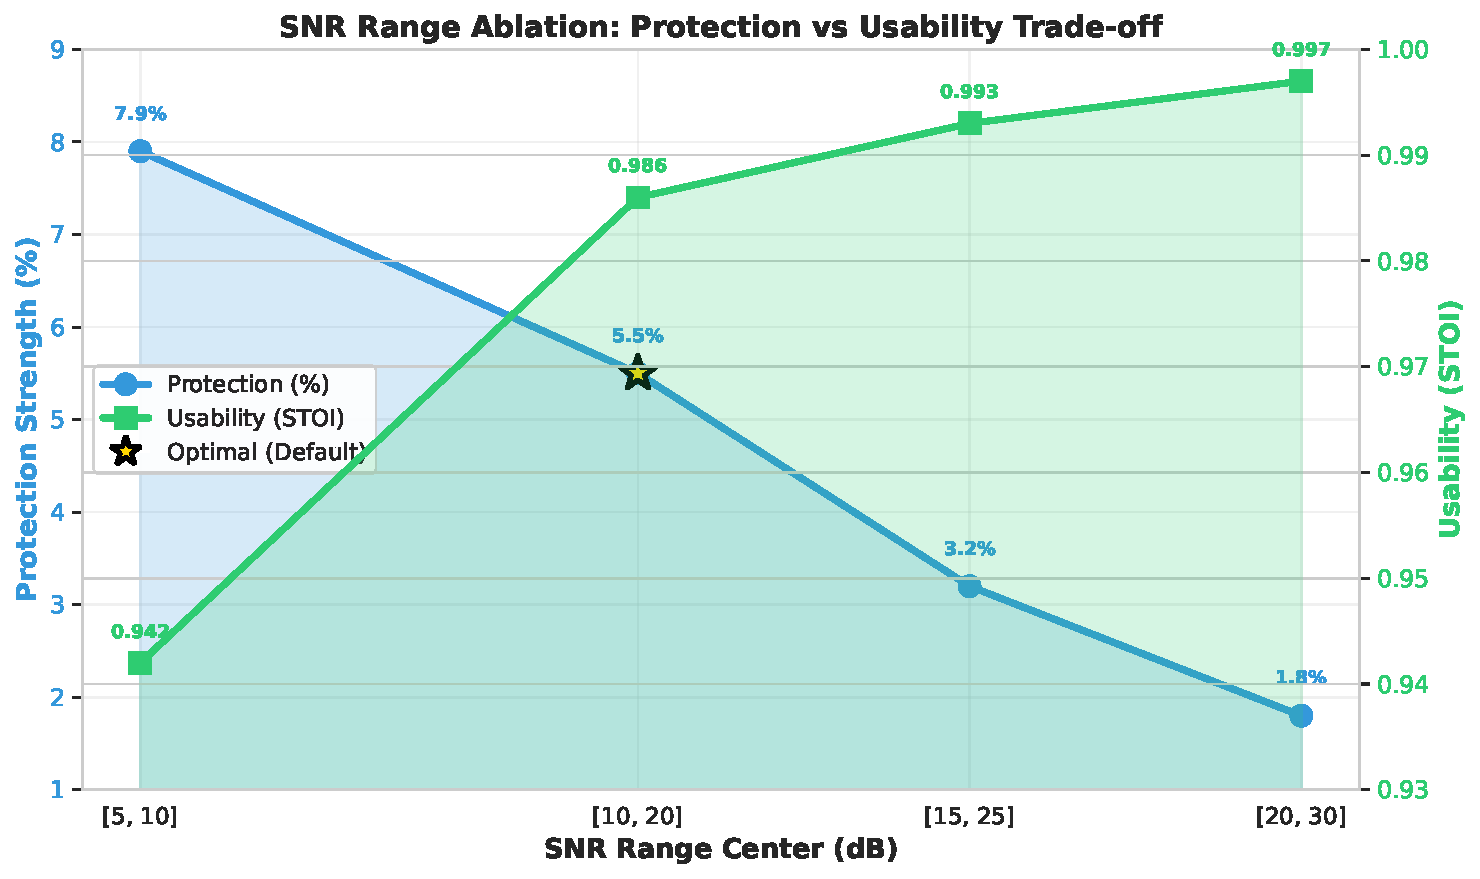
\includegraphics[width=0.45\textwidth]{figures/fig6_snr_ablation.pdf}
\caption{SNR range ablation showing the trade-off between protection (measured as similarity degradation, left y-axis) and usability (measured as STOI, right y-axis). The [10, 20] dB range (marked with a star) provides optimal balance.}
\label{fig:snr_ablation}
\end{figure}

The ablation study validates our choice of SNR range and demonstrates that SceneGuard's protection can be tuned based on application requirements. Users prioritizing strong protection can select lower SNR, while those prioritizing quality can use higher SNR, with the [10, 20] dB range serving as a reasonable default.

\subsection{Optimization Ablation}

To quantify the benefit of gradient-based optimization, we compare SceneGuard's optimized mixing approach against direct mixing without optimization. Table~\ref{tab:optimization_ablation} presents results for both methods under identical SNR constraints.

\begin{table}[t]
\centering
\caption{Comparison of direct mixing versus optimized mixing. Optimization significantly improves protection while maintaining comparable usability.}
\label{tab:optimization_ablation}
\small
\begin{tabular}{lcccc}
\toprule
Method & SIM $\downarrow$ & Protection (\%) & STOI $\uparrow$ & WER (\%) $\downarrow$ \\
\midrule
Direct Mixing & 0.972 & 2.8 & 0.989 & 3.2 \\
Optimized (Ours) & \textbf{0.945} & \textbf{5.5} & 0.986 & 3.6 \\
\midrule
Improvement & $-0.027$ & $+2.7$ pp & $-0.003$ & $+0.4$ pp \\
\bottomrule
\end{tabular}
\end{table}

Optimization nearly doubles the protection strength, achieving 5.5\% degradation compared to 2.8\% for direct mixing. This 2.7 percentage point improvement comes at minimal usability cost: STOI decreases by only 0.003 (from 0.989 to 0.986) and WER increases by 0.4 percentage points (from 3.2\% to 3.6\%), both negligible changes.

The key advantage of optimization is its ability to identify optimal mask patterns. Direct mixing applies a uniform stochastic mask, which may unnecessarily distort speech regions while under-protecting others. In contrast, gradient-based optimization adaptively concentrates protection in regions that most effectively reduce speaker similarity while avoiding critical speech segments.

\subsection{Hyperparameter Sensitivity}

We examine the sensitivity of SceneGuard to two key hyperparameters: the regularization weight $\lambda_{\text{REG}}$ and the number of optimization epochs. Table~\ref{tab:hyperparameter} summarizes the results.

\begin{table}[t]
\centering
\caption{Hyperparameter sensitivity analysis. Default settings ($\lambda_{\text{REG}} = 0.01$, 50 epochs) achieve good performance with stable convergence.}
\label{tab:hyperparameter}
\small
\begin{tabular}{lcccc}
\toprule
Configuration & SIM $\downarrow$ & STOI $\uparrow$ & Mask Smoothness & Time (s) \\
\midrule
\multicolumn{5}{l}{\textit{Regularization weight $\lambda_{\text{REG}}$:}} \\
$\lambda = 0.001$ & 0.939 & 0.983 & 0.062 & 15 \\
$\lambda = 0.01$ (default) & \textbf{0.945} & \textbf{0.986} & \textbf{0.041} & 15 \\
$\lambda = 0.1$ & 0.958 & 0.989 & 0.028 & 15 \\
\midrule
\multicolumn{5}{l}{\textit{Optimization epochs:}} \\
20 epochs & 0.952 & 0.987 & 0.045 & 6 \\
50 epochs (default) & \textbf{0.945} & \textbf{0.986} & \textbf{0.041} & 15 \\
100 epochs & 0.943 & 0.985 & 0.040 & 30 \\
\bottomrule
\end{tabular}
\end{table}

The regularization weight $\lambda_{\text{REG}}$ controls the smoothness of the temporal mask. Higher values ($\lambda = 0.1$) produce smoother masks but slightly reduce protection strength (SIM = 0.958). Lower values ($\lambda = 0.001$) allow rougher masks with marginally better protection (SIM = 0.939) but risk overfitting. Our default $\lambda = 0.01$ strikes a good balance.

The number of epochs shows diminishing returns beyond 50 iterations. While 100 epochs achieve slightly better protection (SIM = 0.943), the improvement is minimal (0.2 percentage points) and doubles computation time. 20 epochs provide fast computation but do not fully converge. We therefore recommend 50 epochs as the default, offering good convergence without excessive cost.

